\documentclass[11pt,a4paper]{article}
\usepackage[T1]{fontenc}
\usepackage{graphicx}
\usepackage{mathtools}
\usepackage{amssymb}
\usepackage{geometry}
\usepackage{titlesec}
\usepackage{enumitem} % 添加enumitem宏包
\usepackage{amsfonts}
\usepackage{amssymb}
\usepackage{fancyhdr} % 添加fancyhdr宏包
\usepackage{lastpage} % 添加lastpage宏包
\usepackage{graphicx} % 导入graphicx包
\usepackage{gensymb} % 引入gensymb包
\usepackage[UTF8]{ctex}
% 应用fancyhdr宏包的页脚样式
\pagestyle{fancy}
\fancyhf{} % 清除当前的页眉页脚设置
\fancyfoot[L]{免费开源,请勿商用} % 页脚左下方显示文字
\fancyfoot[R]{作者:阿尧} % 页脚右下方显示文字
\renewcommand{\headrulewidth}{0pt} % 去掉页眉的横线
\renewcommand{\footrulewidth}{1pt} % 设置页脚的横线宽度
\usepackage{draftwatermark} %增加水印
\SetWatermarkText{本真题由b站up陈瀚尧探索世界免费开源}
\SetWatermarkScale{0.3} % 可以调整为合适的大小
\SetWatermarkColor{gray!50} % 灰色透明度为50%

% 设置更窄的页面边距
\geometry{left=3cm, right=3cm, top=1cm, bottom=2cm}

% 设置section标题格式
\titleformat{\title}{\bfseries}{\thetitle}{1em}{}

% 设置section之间的距离
\titlespacing*{\section}{0pt}{3.25ex plus 1ex minus .2ex}{1.5ex plus .2ex}

\begin{document}
    \title{中国科学院大学\\2021年招收攻读硕士学位研究生入学统一考试试题\\科目名称:光学}
    \author{制作者:b站up 陈瀚尧探索世界}
    \date{}
    \maketitle
    % 设置section标题不显示序号
    \titleformat{\section}[block]{\normalfont\Large\bfseries}{}{0pt}{}

    % 设置itemize环境的项目符号为空
    \setlist[itemize]{label=} 

    \section{考试须知:}
    \begin{itemize}[topsep=0pt,itemsep=0pt,partopsep=0pt]
        \item 1.本试卷满分为150分,全部考试时间总计180分钟。
        \vspace{-3mm}
        \item 2.所有答案必须写在答题纸上,写在试题纸上或草稿纸上一律无效。
        \vspace{-3mm}
        \item 3.可以使用无字典存储或编程功能的电子计算器。(此条对于25考研可能作废)
    \end{itemize}
    \vspace{-5mm}
    \noindent\rule{\textwidth}{0.5pt} % 添加一条线
    \vspace{-12mm}
    \subsection*{1.写出光波场$E_x=E_0\cos (\omega t-kz)$,$E_y=E_0\cos (\omega t-kz+\frac{\pi}{4})$的复数表达式和琼斯矩阵矢量表达式,并确定其偏振状态。}
    \vspace{15mm}
    \subsection*{2.一束自然光由红宝石$(n=1.76)$以布儒斯特角斜入射到空气中,试求界面反射率、透射率及反射光、透射光的偏振度。}
    \vspace{15mm}
    \subsection*{3.太阳直径对地球表面的张角$2\theta$约为$0\degree32'$,如图1所示。在暗室中若直接用太阳光作光源进行双缝干涉实验(不限制光源尺寸的单缝),则双缝间距不能超过多大?(设太阳光的平均波长$\lambda =0.55\mu m$,日盘上各点的亮度差可以忽略。)}
    \vspace{15mm}
    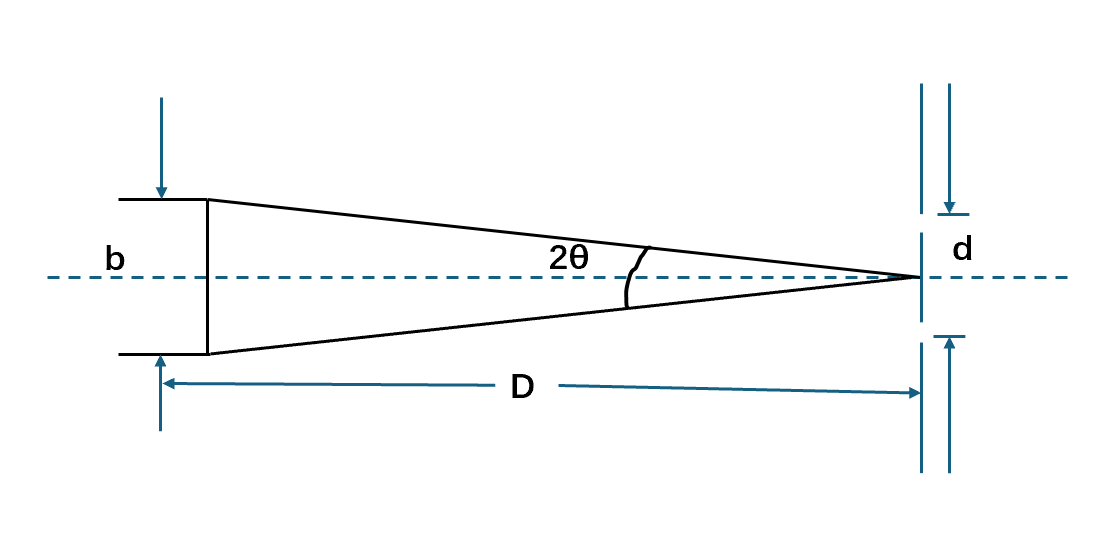
\includegraphics[scale=0.5]{1.jpg}% 插入图片,按50%的比例缩放
    \subsection*{4.已知F-P标准具的空气间隔$h=2cm$,两镜面反射率均为$R=90\%$。试确定其对$\lambda =632.8nm$红光的分光特性。}
    \vspace{15mm}
    \subsection*{5.电子显微镜的孔径角为$2\mu =8\degree$,电子束的波长为$10nm$,试求其最小分辨距离。若人眼在明视距离处能分辨$67\mu m$的距离,则此显微镜的放大倍数是多少?}
    \vspace{15mm}
    \subsection*{6.单色平行光的波长$\lambda =490nm$,透光缝的宽度为$\alpha=10x10^{-4}cm$,不透光缝的宽度$b=2.0x10^{-4}cm$。(1)若单色光垂直照射在光栅上,最多能观察到的明纹总数(包括中央明纹)为多少?(2)若入射单色光与光栅平面法线方向的夹角$\varphi =30\degree$,此时光栅衍射条纹中两侧的最高级次分别为哪一级?}
    \vspace{15mm}
    \subsection*{7.对于钠黄光,晶体的主折射率$n_0=1.6584$,$n_e=1.4864$。图2所示,光束以$60\degree$角入射到该晶体表面,设光轴与晶体表面平行,并垂直于入射面。}
    \begin{itemize}
        \vspace{0mm}
        \item (1)画出o光与e光的光路,并标出其振动方向;
        \vspace{0mm}
        \item (2)求晶体中o光和e光的夹角。
        \vspace{0mm}
    \end{itemize}
    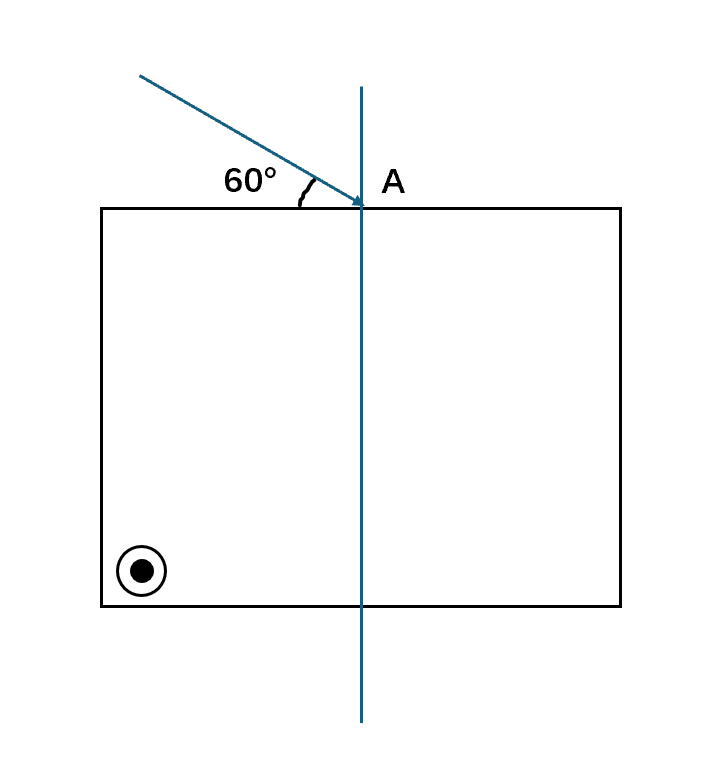
\includegraphics[scale=0.5]{2.jpg}% 插入图片,按50%的比例缩放
    \vspace{15mm}
    \subsection*{8.图中A为纵向运用的电光晶体KDP($n_{o}=1.512$,$\gamma_{63}=10.6x10^{-10}\frac{cm}{V})$,B为厚度$d=10mm$的方解石晶体($n_{o}=1.5246$,$n_{e}=1.4792$,光轴方向与通光面的法线方向成$45\degree$夹角),A、B晶体平行放置,试计算一束波长$\lambda=550nm$的线偏振光(光电场振动方向沿晶体主轴方向)垂直入射KDP时,晶体的半波电压$V_{\frac{\lambda}{2}}$为多大?绘出相应于电压为$V=0$和$V=V_{\frac{\lambda}{2}}$时,A、B晶体的传输光路图及振动方向:计算由B晶体输出的两个光的间距、相位差。}
    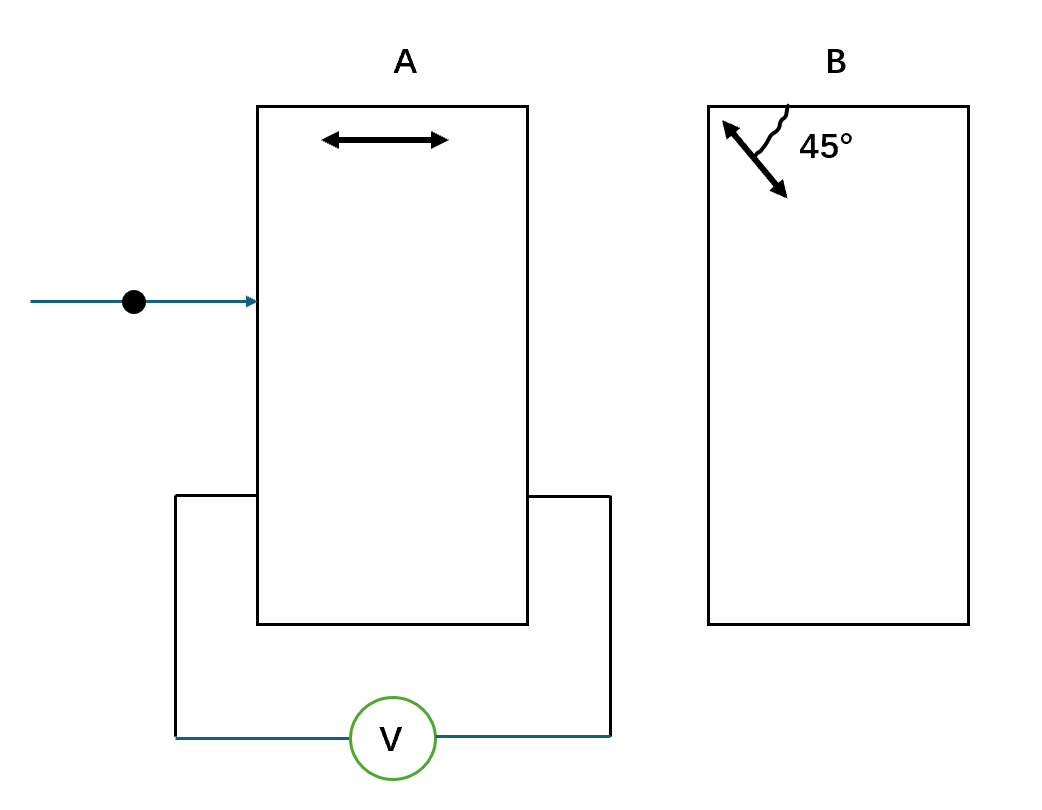
\includegraphics[scale=0.5]{3.jpg}% 插入图片,按50%的比例缩放
    \vspace{15mm}
    \subsection*{9.已知一透镜结构参数如下(单位$mm$):$r_1=10$,$n_1=1.0$,$d_1=5$,$n_2=n_1^{'}=1.5163$,$r_2=-50$,$n_2^{'}=1.0$。高度$y_1=10mm$的物体位于透镜前$l_1=-100mm$处,求像的位置和大小}
    \vspace{20mm}
    \subsection*{10.一组合系统如图所示,薄正透镜的焦距为$20mm$,薄负透镜的焦距为$-20mm$,两单透镜之间的距离为$10mm$,当一个物体位于正透镜前方$100mm$处,求组合系统的放大率和像的位置。}
    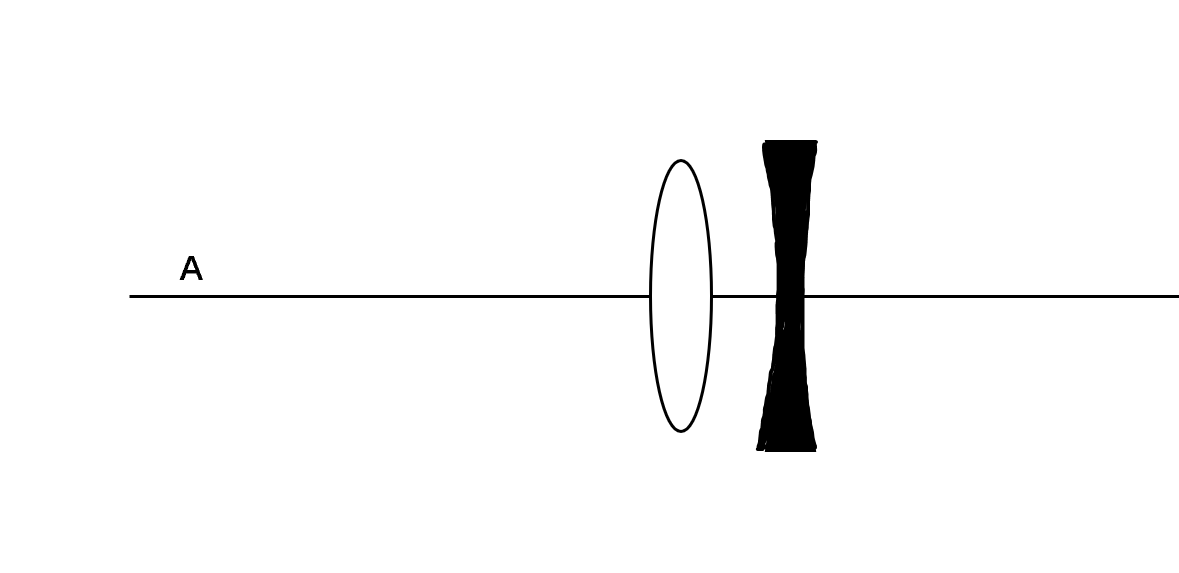
\includegraphics[scale=0.5]{4.jpg}% 插入图片,按50%的比例缩放
    \vspace{15mm}
    \subsection*{11.已知一个光学系统由三个零件组成,透镜1:$f_1^{'}=-f_1^{'}=100mm$,口径$D_1=40mm$;透镜2:$f_2^{'}=-f_2^{'}=120mm$,口径$D_2=30mm$,它和透镜1之间的距离为$d_1=20mm$,光阑3口径为$20mm$,它和透镜2之间的距离$d_2=30mm$。物点A的位置$L_1=-200mm$,试确定该光组中,哪一个光孔是孔径光阑,哪一个是视场光阑?}
    \vspace{20mm}
    \subsection*{12.欲将一架-250倍的显微镜改装为望远镜,已知显微镜物镜的焦距为$10mm$,物镜到目镜的焦距$d=230mm$,若不改变仪器结构镜筒的长度,且使用显微镜的目镜作为望远镜的目镜,则应该配焦距为多少的物镜?改装后望远镜的放大倍数为多少?}
    \vspace{20mm}
    \subsection*{13.我国于2020年7月23日发射的火星探测卫星,将于2021年抵达火星表面,并开展探测。已知火星半径$R=3396km$,太阳的辐强度为$I=3X10^{25}\frac{W}{sr}$,太阳到火星的平均距离$L=2.28x10^{11}m$,求火星接收的辐通量和辐照度。}
    \vspace{20mm}
\end{document}